%%
%% Suspensions chapter
%%
%% Author:
%% Version:
%%
%\documentclass[color,cite,epsfig,12pt]{article}
%\usepackage{graphicx}
%\usepackage{placeins}

%\begin{document}
%%\bibliographystyle{unsrt} 

\subsection{The LIGO active seismic filters}
%%\subsection{The LIGO active seismic filters}
\label{sec:LIGO_filters}

%\emph{Author:  F. Ricci}

In the the Advanced LIGO project the seismic noise suppression problem has been fixed using
a different approach \cite{aLIGO}. The suspension chain has been designed including 
an in-vacuum two-stage active isolation system where the inner modes are reduced by sensing 
the stage motion and applying forces in feedback loops. 

The in-vacuum attenuator provides isolation above about 0.2 Hz and consists of two-stages 
platforms connected to each other by springs. Each stage is supported by three maraging 
steel blade springs and short pendulums from the stage above it to provide vertical and 
horizontal compliance in six degrees of freedom (see fig. \ref{fig:active_filter} left side). 
Contained in each stage are six position sensors and six seismometers which collectively measure 
motion in all degrees of freedom. The signals from these detectors are feed-back to magnetic 
actuators to reduce the motion of the platforms. The rigid body modes of these stages are 
between 1.3 and 7 Hz, while the unity gain frequency of the control loop will be at about 25 Hz. 
Together, these stages provide isolation of about a factor of 300 at 1 Hz and about 3000 at 10 Hz, 
in amplitude. The second stage contains an optical table, from which the suspension and test 
mass are supported.

\begin{figure}[htbp!]
\centering
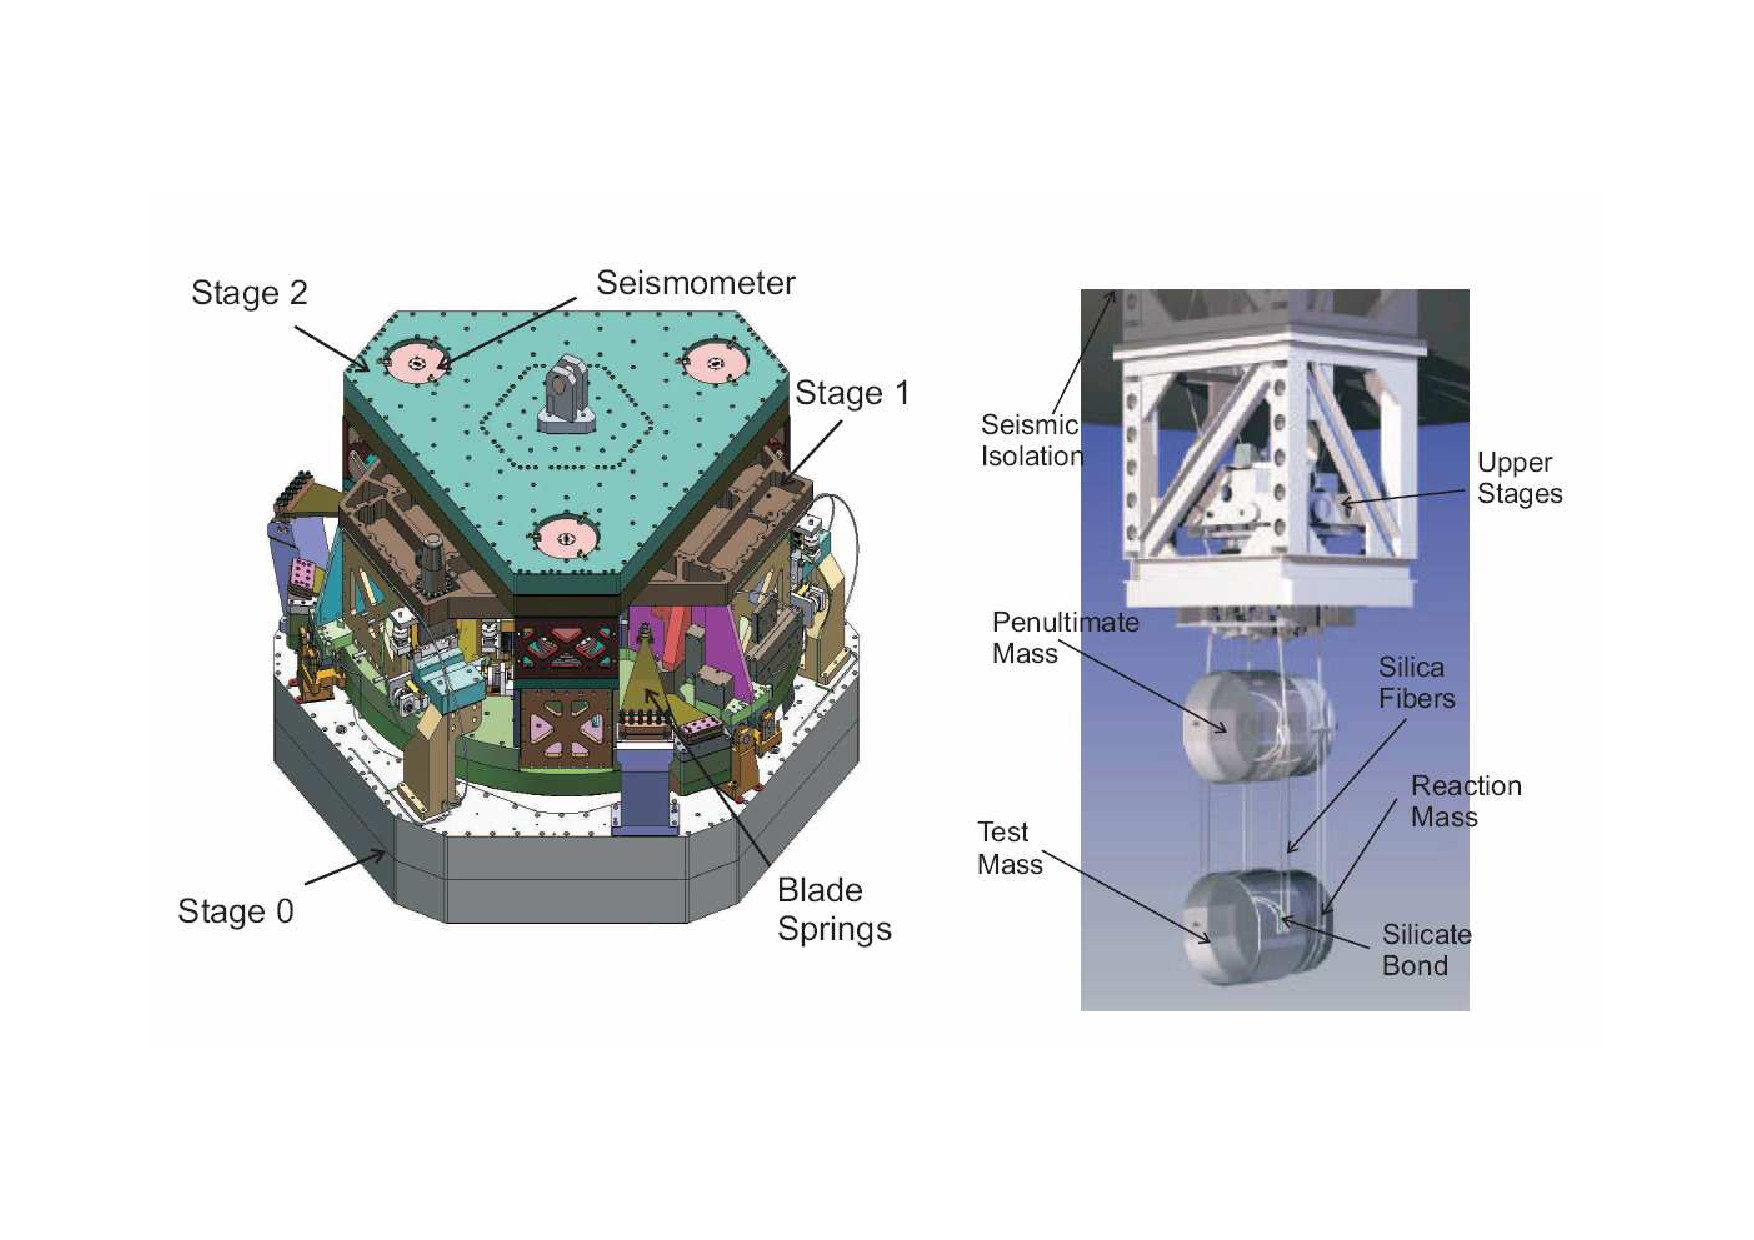
\includegraphics[width=14cm]{./Sec_Suspensions/Figures/Active_filter_2.pdf}
\caption{Internal stages of the large vacuum chamber seismic isolation system (left side).
Advanced LIGO suspension: the test mass connected at the bottom to the penultimate mass above
it with silica fibers. On right side, the reaction mass behind the test mass is visible}
\label{fig:active_filter}
\end{figure}

The Advanced LIGO test masses will be supported by suspensions that hang below the seismic
isolation platforms. These suspensions are multistage pendulums with a final stage consisting
of the test mass hanging on fused silica fibers. They will provide additional passive isolation,
allow for necessary control forces to be applied without adding excess noise, and minimize the
effect of thermal noise.

In addition to the main quadruple suspension chain that supports the test mass, there will also
be a nearly identical reaction chain placed 5 mm behind it (see fig. \ref{fig:active_filter} 
right side). This chain will allow control forces for global angular and longitudinal degrees 
of freedom to be applied from a quiet platform. These forces will be hierarchically used, 
with large forces applied with coils and magnets between both the upper intermediate and 
penultimate masses but with fine control forces applied with an electrostatic drive (ESD). 
The ESD is a gold pattern deposited on the face of the final reaction mass and applies 
forces to the test mass with an electrostatic field.
Local damping of all the low frequency suspension modes will be done with co-located sensors
and actuators on the top mass to insure that any sensing noise will be well isolated from the
test mass.

\noindent
The main feature of this suspension, shorter than the Virgo Superattenuator, is represented by 
the fact that the final isolation requirements are reached with a system based mainly on an 
active hierarchical control.


%\end{document}

